\section{Une épidémie (7 points)}

Une épidémie affecte une île du Pacifique, depuis le mois d'avril 2013. Nous disposons des données du nombre de personnes infectées sur les mois d'avril à septembre 2013. Ces données sont récapitulées dans le tableau suivant :

\vspace*{0.5cm} 
\begin{center}
	\begin{tabular}{|@{\ }l@{\ }|@{\ }c@{\ }|@{\ }c@{\ }|@{\ }c@{\ }|@{\ }c@{\ }|@{\ }c@{\ }|@{\ }c@{\ }|}
		\hline
		Mois                                & Avril      & Mai        & Juin & Juillet    & Août & Septembre \\ \hline
		Rang du mois $x_i$                  & 0          & 1          & 2    & 3          & 4    & 5         \\ \hline
		Nombre de malades en milliers $y_i$ & \num{17.5} & \num{27.5} & 35   & \num{42.5} & 49   & 51        \\ \hline
	\end{tabular}
\end{center}

\begin{questions}
	\question[1] En observant le nuage de points correspondant au tableau, tracé ci-dessous, un ajustement affine est-il envisageable ?
	
	\question[1\half] Calculer les coordonnées du point moyen $G$ du nuage de points et l'ajouter sur le nuage de points.
	
	\question[2] On considère la droite $(d)$, d'équation $y = \num{6.8} x + 20$, réalise un bon ajustement du nuage de points. Tracer la droite $(d)$.
	
	\question En utilisant l'approximation affine précédente, déterminer par le calcul :
	\begin{parts}
		\part[1\half] le nombre de personnes atteintes en février 2014 ;
		\part[1\half] le mois à partir duquel la population atteinte dépassera 100 00 personnes.
	\end{parts}
	
\end{questions}

\begin{center}
	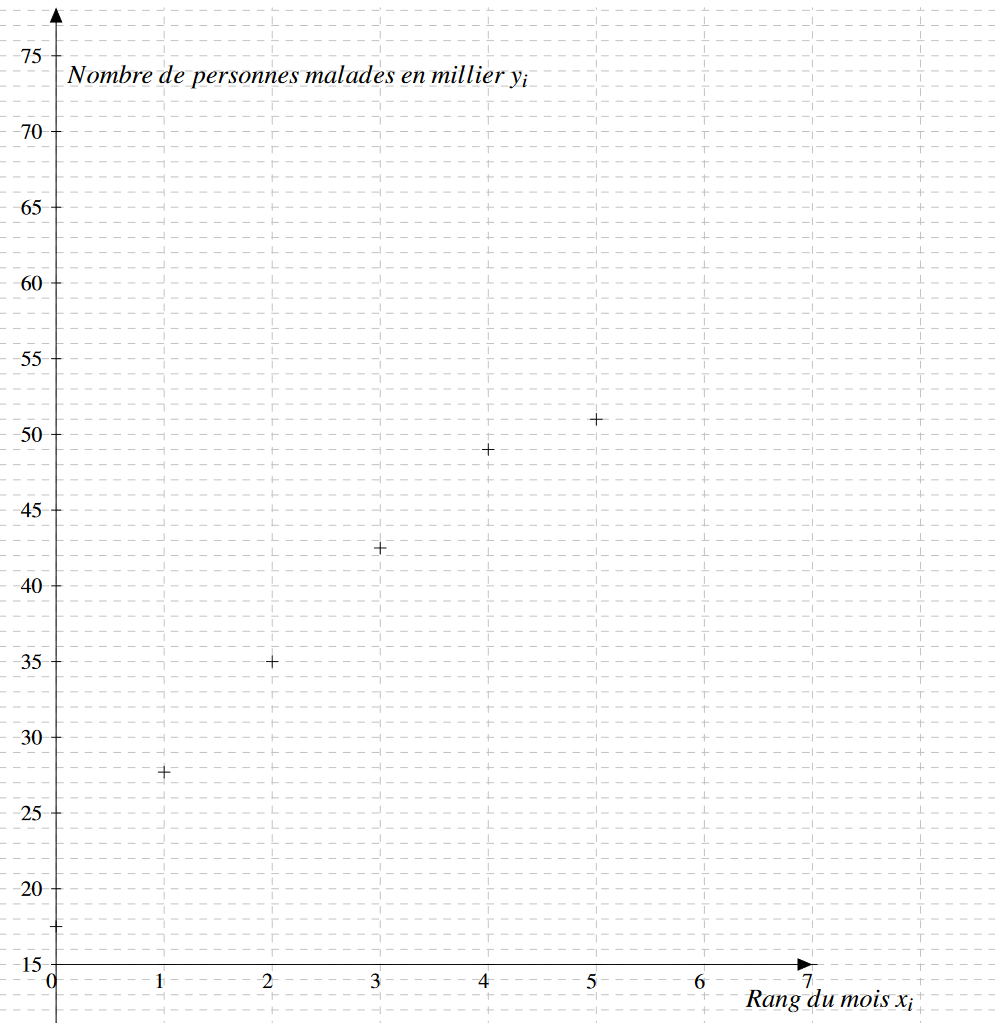
\includegraphics[scale=0.5]{nuage}
\end{center}